\documentclass[demonstration]{jfsma}

\usepackage[T1]{fontenc}
\usepackage{graphicx}
%\usepackage{color}
%\renewcommand\UrlFont{\color{blue}\rmfamily}
\usepackage{amsthm}
\usepackage{amsmath,amssymb,amsfonts}
\usepackage{tabularx}
\usepackage{caption}
\usepackage{listings}
% \usepackage{titlesec}
% \usepackage[english]{babel}
% \captionsetup{font=it}
\usepackage{ragged2e}
\usepackage{xurl}
\usepackage{hyperref}
\usepackage{pifont}
\usepackage{footmisc}
\usepackage{multirow}
\usepackage{enumitem}
\usepackage{algorithm2e}
\usepackage{float}
\usepackage{listings}
\usepackage{xcolor}
% \usepackage[inline, shortlabels]{enumitem}
% \usepackage[hyphens]{url}

\definecolor{codegreen}{rgb}{0,0.6,0}
\definecolor{codegray}{rgb}{0.5,0.5,0.5}
\definecolor{codepurple}{rgb}{0.58,0,0.82}
\definecolor{backcolour}{rgb}{0.95,0.95,0.92}
 
\lstdefinestyle{mystyle}{
    backgroundcolor=\color{backcolour},   
    commentstyle=\color{codegreen},
    keywordstyle=\color{magenta},
    numberstyle=\tiny\color{codegray},
    stringstyle=\color{codepurple},
    basicstyle=\footnotesize,
    breakatwhitespace=false,         
    breaklines=true,                 
    captionpos=b,                    
    keepspaces=true,                 
    numbers=left,                    
    numbersep=5pt,                  
    showspaces=false,                
    showstringspaces=false,
    showtabs=false,                  
    tabsize=2
}

\lstset{style=mystyle}

% --- Tickz
\usepackage{physics}
\usepackage{amsmath}
\usepackage{tikz}
\usepackage{mathdots}
\usepackage{yhmath}
\usepackage{cancel}
\usepackage{color}
\usepackage{siunitx}
\usepackage{array}
\usepackage{multirow}
\usepackage{amssymb}
\usepackage{gensymb}
\usepackage{tabularx}
\usepackage{extarrows}
\usepackage{booktabs}
\usetikzlibrary{fadings}
\usetikzlibrary{patterns}
\usetikzlibrary{shadows.blur}
\usetikzlibrary{shapes}

% ---------
% \usepackage{titlesec}
\usepackage{pdfpages}
\usepackage{booktabs}
\usepackage{csquotes}
\usepackage{lipsum}  
\usepackage{arydshln}
\usepackage{smartdiagram}
\usepackage[inkscapeformat=png]{svg}
\usepackage{textcomp}
\usepackage{tabularray}\UseTblrLibrary{varwidth}
\usepackage{xcolor}
\def\BibTeX{{\rm B\kern-.05em{\sc i\kern-.025em b}\kern-.08em
    T\kern-.1667em\lower.7ex\hbox{E}\kern-.125emX}}
\usepackage{cite}
\usepackage{amsmath}
\newcommand{\probP}{\text{I\kern-0.15em P}}
\usepackage{etoolbox}
\patchcmd{\thebibliography}{\section*{\refname}}{}{}{}

\setlength\tabcolsep{0.5pt}

\newcommand{\before}[1]{\textcolor{red}{#1}}
\newcommand{\after}[1]{\textcolor{green}{#1}}

\newcommand{\old}[1]{\textcolor{orange}{#1}}
\newcommand{\rem}[1]{\textcolor{red}{#1}}
\newcommand{\todo}[1]{\textcolor{orange}{\newline \textit{\textbf{TODO:} #1}} \newline \newline }

\newcommand{\jp}[1]{\textbf{\color{red} JPJ: #1}}

\newcounter{relation}
\setcounter{relation}{0}
\renewcommand{\therelation}{\arabic{relation}}
\newcommand{\relationautorefname}{Relation}

\newenvironment{relation}[1][]{%
    \refstepcounter{relation}%
    \noindent \raggedright \textit{\textbf{Relation. \therelation}} \hfill$}
{%
$ \hfill \phantom{x}

}

\newcounter{proof}
\setcounter{proof}{0}
\renewcommand{\theproof}{\arabic{proof}}
\newcommand{\proofautorefname}{Proof}

\renewenvironment{proof}[1][]{
    \refstepcounter{proof}
    \noindent \raggedright \textit{\textbf{Proof. \theproof}}

    \setlength{\leftskip}{1em}

}
{

\
\setlength{\leftskip}{0pt}
}


\titre{Un Outil pour la Conception de SMA par Apprentissage par Renforcement et Modélisation Organisationnelle}


\auteur{Julien Soulé\up{a,b}}{julien.soule@lcis.grenoble-inp.fr}
\auteur{Jean-Paul Jamont\up{a}}{jean-paul.jamont@lcis.grenoble-inp.fr}
\auteur{Michel Occello\up{a}}{michel.occello@lcis.grenoble-inp.fr}
%%%Si besoin d'ajouter des auteurs à la ligne :
\auteurSuite{Louis-Marie Traonouez\up{b}}{louis-marie.traonouez@thalesgroup.com}
\auteurSuite{Paul Théron\up{c}}{paul.theron@orange.fr}

\institution{\up{a}%
  Univ. Grenoble Alpes, Grenoble INP, LCIS, 26000, Valence, France}
\institution{\up{b}%
  Thales Land and Air Systems, BL IAS, Rennes, France}
\institution{\up{c}%
  AICA IWG, La Guillermie, France}

% TODO: est-ce qu'on peut utiliser "dissemination" alors que le papier AIAI n'est pas publié à proprement parler?

\begin{document}

\maketitle

\begin{resume}

% Contexte
L'organisation d'un SMA peut être vue tant du point de vue des interactions individuelles des agents que des schémas collectifs à un niveau plus global.
La recherche d'une organisation permettant d'atteindre un objectif sous des contraintes données ou environnementales est centrale dans la conception d'un SMA.
% Elle englobe différentes relations du niveau individuel comme les interactions avec l'environnement jusqu'au niveau social commme les stratégies collectives. 
%
% Problème
Une approche empirique pour trouver une organisation adéquate dans certains environnements complexes peut s'avérer coûteuse.
%
% Contribution
Nous proposons PRAHOM qui augmente le framework de simulation PettingZoo pour suggérer des spécifications organisationnelles susceptibles de guider la conception vers un SMA adéquat.
% en reliant modèle organisationnel et apprentissage par renforcement.
% \jp{tu dis trop de choses dans une meme phrase. On s'attend a ce que tu dises en 1er a quoi ca sert. Apres si tu penses que c'est important a ce niveau l'integration des contraintes dit le ensuite}
Il intègre des contraintes dans l'apprentissage et génère de spécifications organisationnelles en utilisant les comportements des agents entraînés.
% Les spécifications générées peuvent guider le concepteur.

\end{resume}

\motscles{Organisations, Ingénierie multi-agents, Apprentissage multi-agent}

\bigskip

\begin{abstract}

% Context
The MAS organization can be seen both from the point of view of individual agents' interactions or through the collective patterns at a global level. Searching for an organization that allows achieving a goal under given or environmental constraints is central in MAS design.
%
% Issue
An empirical approach to finding a suitable organization in some environments can be costly.
%
% Contribution
We propose PRAHOM which augments the PettingZoo simulation framework to suggest organizational specifications likely to guide the design towards a suitable MAS.
It integrates constraints into learning and generates organizational specifications using the trained agents' behaviors.
% The generated specifications can guide the designers.

\end{abstract}

\keywords{Organizations, Multi-agent engineering, Multi-agent learning}

\section{Introduction}



% Contexte:


%% Introduire le concept de SMA de Cyberdefense en le supportant par l'AICA
% Introduire la problématique de la conception de SMA en général à partir de ce cas précis


% Un agent AICA~\cite{Kott2023}
%
% (\emph{Autonomous Intelligent Cyberdefense Agent}\footnote{La recherche sur les AICA a été initiée dans le cadre du groupe \emph{NATO IST-152} puis de l'\emph{AICA International Work Group} : \url{https://www.aica-iwg.org/}.})
% %
% doit être déployé sur un environnement en réseaux pour détecter, identifier, caractériser des attaques, élaborer et exécuter des contre-mesures permettant de minimiser les dommages potentiels.
% Un agent AICA peut être vu comme un SMA de Cyberdefense~\cite{Singh2015} où la couverture de Cyberdéfense est distribuée sur un ensemble d'agents de Cyberdéfense collaborant entre eux de façon autonome.

% todo

%\jp{j'aime pas cette attaque de l'article... c'est abrupte... on en parle}
% js : Notre contribution aborde le problème de la conception...
%jpj j'ai pas dit que c'était faut je dis que c'est abrupte
% js : ok donc je garde comme ça ? au moins c'est clair même si c'est pas très joliement écrit
%non michel n'aime pas non plus : on en a parlé hier en réunion
% attend laisse moi lire l'article j'arrive pas a faire abstraction de tes remarques :) et je recommence 
% js : ok, je touche pas et tu m'envoies un message quand tu as fini ?
La conception d'un SMA requiert que le concepteur ait connaissance de l'environnement de déploiement afin de proposer des logiques internes aux agents susceptibles  de leur permettre d'atteindre collectivement l'objectif donné.
%
Cette connaissance peut s'avérer insuffisante en raison de la complexité de l'environnement ; ou en raison de contraintes d'accès (temporelles, spatiales et légales) limitant les possibilités de sa compréhension empirique.
% \jp{metaproposition : La conception d'un SMA demande d'avoir une bonne connaissance de l'environnement de déploiement car ... . Dans beaucoup d'applicaitons notamment ... l'environnement est ....}
% La flexibilité d'un SMA de Cyberdéfense renforce sa résilience en lui permettant de s'adapter continuellement aux contraintes de l'environment tout en respectant des politiques de sûreté. Les aspects organisationels sont considerés dans l'ingénierie d'un tel SMA au sein des travaux de recherche.

%% Elargir le sujet des SMAC/AICA au contexte des SMA en général

% \jp{verifier que ca fait sens apres reformulation "ce probleme"}
Concevoir un SMA peut être vu au travers de l'\textbf{organisation} que nous voyons comme l'ensemble des \textbf{politiques} des agents
\footnote{Une politique est une relation entre observations et actions.}
considérées tant du point de vue individuel que du point de vue global. Les mécanismes organisationnels induits par ces politiques peuvent être explicités au travers de \textbf{modèles organisationnels}.

% \jp{Question qui se posera : on dit qu'on ne connaît pas (ou très mal) l'environnement et du coup on fait de l'apprentissage sur un environnement simulé}


% le \textbf{support organisationel} qui explicite comment les agents coordonnent leurs activités pour atteindre de manière collaborative un objectif commun.
La conception d'un SMA devient alors la recherche d'une organisation permettant d'atteindre l'objectif donné de façon optimale sous des contraintes environnementales
\footnote{Approche développée dans l'article \textquote{Une Approche basée sur l'Apprentissage par Renforcement pour l'Ingénierie Organisationelle d'un SMA} soumis pour JFSMA 2024 }.
Même si la plupart des méthodes de conception telles que GAIA~\cite{Cernuzzi2014} ou KB-ORG~\cite{Sims2008} facilitent la recherche d'une organisation adéquate pour un environnement et un objectif donné~\cite{Mefteh2013} ; elles ne permettent pas d'automatiser totalement la recherche des politiques des agents satisfaisant les exigences données et explicitant l'organisation.

Nous introduisons \emph{PRAHOM Wrapper} (Partial Relations with Agent History and Organization Model Wrapper), une couche logicielle pour le framework de simulation Multi-Agent \emph{PettingZoo} qui permet de :
%
i) Entraîner les politiques des agents à atteindre un objectif donné dans un environnement et en respectant d'éventuelles spécifications organisationnelles ;\quad
ii) Déterminer des spécifications organisationnelles %\MO: à partir% 
en analysant le comportement des agents entraînés.
%
% \jp{tu dis "vise" dont l'objectif mais ce n'est pas l'objectif que tu donnes ici c'est le moyen}
Pour cela, il combine un processus MARL (Multi-Agent Reinforcement Learning) avec le modèle organisationnel $\mathcal{M}OISE^+$~\cite{Hubner2007}.

% La section II résume d'abord les concepts fondamentaux sur lesquels est construit \emph{PRAHOM Wrapper}.
La section II donne un aperçu du positionnement de \emph{PRAHOM Wrapper} parmi les travaux existants.
La section III  présente les fonctionnalités offertes par \emph{PRAHOM Wrapper} et son utilisation au travers d'un environnement de type jeu Atari.
La section IV conclut sur \emph{PRAHOM Wrapper} en discutant de ses limitations et des travaux futurs.

% ================================================== =================================================== =

% \section{Concepts fondamentaux}

% Nous présentons les bases du modèle organisationnel $\mathcal{M}OISE^+$ et les bases MARL sur lesquelles est construite \emph{PRAHOM Wrapper}.

% \subsection{Modèle organisationnel $\mathcal{M}OISE^+$}

% $\mathcal{M}OISE^+$~\cite{Hubner2007} permet de caractériser une organisation selon trois types de spécifications :

% Les \textbf{spécifications structurelles} décrivent les moyens que les agents peuvent exploiter pour atteindre un objectif. Il comprend l'ensemble des \emph{rôles}, des sous-groupes, des \emph{liens} intra et inter groupe, des \emph{compatibilités} intra et inter groupe, ainsi que les \emph {cardinalités} des rôles et des sous-groupes.
% % Un \emph{lien} indique si deux rôles sont liés en raison de liens de connaissance, de communication ou d'autorité. Une \emph{compatibilité} indique si deux rôles peuvent être adoptés par le même agent. Les \emph{cardinalités} de rôle et de sous-groupe font respectivement référence au nombre minimal et maximal de rôles et de sous-groupes.

% Les \textbf{spécifications fonctionnelles} décrivent la manière d'atteindre un objectif. Il comprend entre autres des \emph{objectifs} globaux, des \emph{missions}, des \emph{plans} et la cardinalité des agents engagés dans une mission.

% Les \textbf{spécifications déontiques} permettent de relier les spécifications fonctionnelles et structurelles à travers un ensemble de \emph{permissions} et d'\emph{obligations} durant des périodes déterminées.
% % Une \emph{permission} signifie qu'un agent jouant le rôle $\rho_a$ est autorisé à s'engager dans la mission $m$ pour une contrainte de temps donnée $tc$. De même, une \emph{obligation} signifie qu'un agent jouant le rôle $\rho_a$ doit s'engager dans la mission $m$ pour une contrainte de temps donnée $tc$. Une contrainte de temps $tc $ spécifie un ensemble de périodes déterminant si une autorisation ou une obligation est valide.


% \subsection{Apprentissage par Renforcement Multi-agent}

% Cela pousse les agents à converger vers des mécanismes de coopération, des stratégies collectives, etc.

% Nous utilisons le modèle Markovien \emph{Dec-POMDP} (Decentralized-Partially Observable Markov Decision Process)~\cite{Oliehoek2016} pour modéliser un environnement et appliquer des techniques MARL. En effet, il considère plusieurs agents de façon analogue à un SMA. Il permet de modéliser l'incertitude de l'environnement pour les changements induits par les actions, les observations reçues. Sa fonction de récompense est commune aux agents ce qui favorise la formation d'actions orientées pour la collaboration~\cite{Beynier2013}.
% % Formellement, un Dec-POMDP est un 7-tuple $(S,\{A_i\},T,R,\{\Omega_i\},O,\gamma)$ , où : $S = \{s_1, .. s_{|S|}\}$ est l''ensemble des états possibles ; $A_{i} = \{a_{1}^{i},..,a_{|A_{i}|}^{i}\}$ l'ensemble des actions possibles pour l'agent $i$ ; $T$ pour que $T(s,a,s') = \probP{(s'|s,a)}$ l'ensemble des probabilités de transition conditionnelles entre les états ; $R : S \times A \times S \rightarrow \mathbb{R}$ la fonction de récompense ; $\Omega_{i} = \{o_{1}^{i},..,o_{|\Omega_{i}|}^{i}\}$  l'ensemble d'observations pour l'agent $ag_i$ ; $O$ pour que $O(s',a,o) = \probP{(o|s',a)}$  l'ensemble des probabilités d'observation conditionnelles ; $\gamma \in [0,1]$, le facteur de remise.

% Nous appelons \textbf{résoudre}/\textbf{résoudre sous-optimalement} le Dec-POMDP pour une équipe, la recherche d'une politique conjointe permettant de maximiser/dépasser un seuil de récompense cumulée sur un horizon fini.

% % ============================================================================



\section{Travaux et positionnement}

Le MARL est un paradigme d'apprentissage automatique où les agents apprennent à prendre des décisions en interagissant avec un environnement. L’objectif est qu'un ensemble d'agents maximisent la récompense cumulée au fil du temps grâce à un processus d’essais et d’erreurs.
Le MARL permet de converger automatiquement vers des politiques permettant d'atteindre l'objectif donné. Réinterpréter ces politiques individuelles en des spécifications organisationnelles demande un travail d'explicabilité à un niveau collectif peu abordé dans la littérature.
% \jp{de l'explicabilité seulement ou aussi des aspects organisationnel... si c'est les deux il faut revoir "la question de l'organisation et en particulier de son explicabilité"}.
% On présente l'aperçu des travaux connexes identifiés en trois catégories.
% je fais des modifications dans le texte : il faudra que tu relises comme il faut :)

\paragraph{\textbf{Cadres pour MARL avec aspects organisationnels}}
%
% \jp{verifier que AAAAA et al. est bien singulier}
% \jp{peut etre commencer par une phrase qui explique ce qu'on appel cadre pour MARL avec aspects organisationnels. Les autres (les 2 paragraph qui s uivent me paraissent plus explicites}
Certains frameworks proposés tentent d'inclure des concepts organisationnels dans le cadre du MARL.
Kazhdan et. al.~\cite{Kazhdan2020} présentent une bibliothèque pour améliorer l'explicabilité des systèmes MARL en les rapprochant de modèles symboliques, notamment pour inférer des rôles.%todo
% \jp si Kazhdan ne s'interesse pas aux organisations c'est maladroit}
%
Wang et. al.~\cite{Wang2020} introduisent une approche dans laquelle les rôles émergents similaires sont poussés à se spécialiser conjointement sur des tâches spécifiques.
% \jp{les role se specialise eux meme ???} conjointement.
%
% Tosic et. al~\cite{Tosic2010} propose un cadre pour la coordination en s'appuyant sur les capacités de communication des systèmes multi-agents.
%
% Zheng et. al.~\cite{Zheng2018} a présenté une plateforme pour MARL qui vise à faciliter la recherche sur l'intelligence collective artificielle en fournissant un ensemble complet dde mesures d'évaluation pour comparer les performances d'algorithmes MARL.

\paragraph{\textbf{Caractérisation des stratégies collectives émergentes}}
%
Heuillet et. al.~\cite{Heuillet2022} proposent une approche pour expliquer les stratégies coopératives en utilisant les valeurs de Shapley. Son efficacité a été démontrée dans le contexte d'applications sur des environnements multi-agents à particules en  expliquant certaines décisions prises. 
%
Jaques et. al.~\cite{Jaques2019} proposent un mécanisme pour tirer profit de la communication entre agents en récompensant les agents ayant une influence causale sur les autres agents. Cette approche conduit à des protocoles de communication appris permettant d'avoir un comportement collectif globalement plus performant.
% \jp{adaptatif? pcq dans l'absolue un comportement collectif plus diversifié on s'en fout}.
% js: globalement plus performant (cf. https://arxiv.org/abs/1810.08647)

\paragraph{\textbf{Adaptation du MARL pour répondre à des exigences}}
%
% Shao et. al.~\cite{Shao2022} introduit une approche reposant sur le modèle leader-follower comme un mécanisme pour améliorer les tâches coopératives multi-agents avec des caractéristiques dynamiques, visant à améliorer l'adaptabilité et la généralisation des systèmes MARL.
%
% Roy et. al.~\cite{Roy2020} présente deux méthodes de régularisation de politiques visant à améliorer la coordination dans l’apprentissage par renforcement.
% %
Le \emph{Specification-Guided Reinforcement Learning} visent à générer les politiques accomplissant une tâche spécifique en utilisant des spécifications externes pour guider l'apprentissage dans l'atteinte d'un objectif et sous des contraintes données~\cite{Bansal2022}.%~\cite{Jothimurugan2023}%
%\jp{ca veut dire que ca sert pour l'identificiation/caracterisation de SMA ?}
%
%
~Jothimurugan et. al.~\cite{Jothimurugan2021} proposent l'apprentissage par spécifications logiques comme l'exploitation de la structure compositionnelle des spécifications pour générer des politiques pour des tâches complexes.

À la différence de ces travaux, notre originalité est d'utiliser explicitement un modèle organisationnel comme moyen général d'exprimer les politiques à un niveau collectif et/ou contraindre leur apprentissage vis-à-vis d'exigences.
% \jp{je me pose la question du "ou" ou du "et"}
% "ou" non exclusif, sinon je peux mettre et/ou si tu penses qu'on comprendrait mieux

% A notre connaissance, il n'existe pas de travaux utilisables pour générer des spécifications organisationelles d'un SMA atteignant un objectif donné sur un environnement et respectant d'éventuelles contraintes d'organisation additionnelles.


% ============================================================================

\section{\emph{PRAHOM Wrapper}}

\subsection{Vue d'ensemble}

\begin{figure}[h!]
  \centering
  


\tikzset{every picture/.style={line width=0.75pt}} %set default line width to 0.75pt        

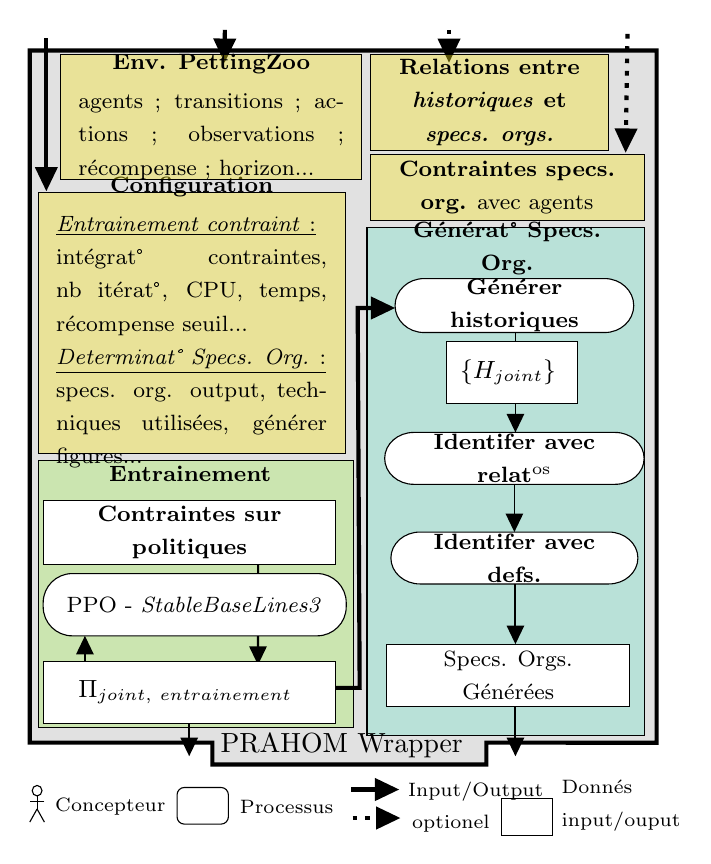
\begin{tikzpicture}[x=0.75pt,y=0.75pt,yscale=-1,xscale=1]
%uncomment if require: \path (0,1656); %set diagram left start at 0, and has height of 1656

%Straight Lines [id:da39585146483301226] 
\draw [fill={rgb, 255:red, 155; green, 155; blue, 155 }  ,fill opacity=0.3 ][line width=1.5]    (262,1077.44) -- (262,1088) -- (130,1088) -- (130,1077.44) -- (42,1077.44) -- (42,998.04) -- (42,744) -- (344,744) -- (344,1077.51) -- cycle ;
%Shape: Rectangle [id:dp15141215707199196] 
\draw  [fill={rgb, 255:red, 184; green, 233; blue, 134 }  ,fill opacity=0.54 ] (46,941.55) -- (197.88,941.55) -- (197.88,1070) -- (46,1070) -- cycle ;
%Shape: Rectangle [id:dp6360114669768389] 
\draw  [fill={rgb, 255:red, 80; green, 227; blue, 194 }  ,fill opacity=0.27 ] (204.48,829.34) -- (338,829.34) -- (338,1073.92) -- (204.48,1073.92) -- cycle ;
%Straight Lines [id:da060910289882972535] 
\draw [line width=0.75]    (118.82,1060.45) -- (118.82,1080.99) ;
\draw [shift={(118.82,1083.99)}, rotate = 270] [fill={rgb, 255:red, 0; green, 0; blue, 0 }  ][line width=0.08]  [draw opacity=0] (8.93,-4.29) -- (0,0) -- (8.93,4.29) -- cycle    ;
%Straight Lines [id:da567561296770805] 
\draw [line width=1.5]    (188.58,1051.05) -- (200.95,1051.05) -- (200,868.05) -- (214,868.05) ;
\draw [shift={(218,868.05)}, rotate = 180] [fill={rgb, 255:red, 0; green, 0; blue, 0 }  ][line width=0.08]  [draw opacity=0] (11.61,-5.58) -- (0,0) -- (11.61,5.58) -- cycle    ;
%Straight Lines [id:da27635620179975406] 
\draw [line width=0.75]    (276,1060.45) -- (276,1081) ;
\draw [shift={(276,1084)}, rotate = 270] [fill={rgb, 255:red, 0; green, 0; blue, 0 }  ][line width=0.08]  [draw opacity=0] (8.93,-4.29) -- (0,0) -- (8.93,4.29) -- cycle    ;
%Straight Lines [id:da08883699834879355] 
\draw [line width=0.75]    (276,992) -- (276,1027) ;
\draw [shift={(276,1030)}, rotate = 270] [fill={rgb, 255:red, 0; green, 0; blue, 0 }  ][line width=0.08]  [draw opacity=0] (8.93,-4.29) -- (0,0) -- (8.93,4.29) -- cycle    ;
%Straight Lines [id:da8779234517114483] 
\draw [line width=1.5]    (136,734) -- (135.88,745.84) ;
\draw [shift={(135.84,749.84)}, rotate = 270.59] [fill={rgb, 255:red, 0; green, 0; blue, 0 }  ][line width=0.08]  [draw opacity=0] (11.61,-5.58) -- (0,0) -- (11.61,5.58) -- cycle    ;
%Straight Lines [id:da43837040952509776] 
\draw [line width=1.5]  [dash pattern={on 1.69pt off 2.76pt}]  (244,734) -- (244,745.84) ;
\draw [shift={(244,749.84)}, rotate = 270] [fill={rgb, 255:red, 0; green, 0; blue, 0 }  ][line width=0.08]  [draw opacity=0] (11.61,-5.58) -- (0,0) -- (11.61,5.58) -- cycle    ;
%Shape: Ellipse [id:dp7999411998489565] 
\draw   (43.18,1100.6) .. controls (43.18,1099.21) and (44.23,1098.08) .. (45.53,1098.08) .. controls (46.83,1098.08) and (47.89,1099.21) .. (47.89,1100.6) .. controls (47.89,1101.99) and (46.83,1103.12) .. (45.53,1103.12) .. controls (44.23,1103.12) and (43.18,1101.99) .. (43.18,1100.6) -- cycle ;
%Straight Lines [id:da7827154744519647] 
\draw    (45.53,1103.12) -- (45.53,1109.43) ;
%Straight Lines [id:da757553550080027] 
\draw    (45.53,1109.43) -- (42,1115.73) ;
%Straight Lines [id:da12186027632053076] 
\draw    (45.53,1109.43) -- (49.06,1115.73) ;
%Straight Lines [id:da8177170825815439] 
\draw    (49.06,1105.64) -- (42,1105.64) ;

%Straight Lines [id:da6711978114234527] 
\draw [line width=1.5]    (196.97,1100.04) -- (215.93,1100.04) ;
\draw [shift={(219.93,1100.04)}, rotate = 180] [fill={rgb, 255:red, 0; green, 0; blue, 0 }  ][line width=0.08]  [draw opacity=0] (11.61,-5.58) -- (0,0) -- (11.61,5.58) -- cycle    ;
%Shape: Rectangle [id:dp565997856178448] 
\draw   (269.27,1104.34) -- (294,1104.34) -- (294,1122) -- (269.27,1122) -- cycle ;
%Rounded Rect [id:dp21323776879671108] 
\draw   (112.97,1102.59) .. controls (112.97,1100.64) and (114.55,1099.06) .. (116.5,1099.06) -- (134.16,1099.06) .. controls (136.11,1099.06) and (137.7,1100.64) .. (137.7,1102.59) -- (137.7,1113.18) .. controls (137.7,1115.13) and (136.11,1116.71) .. (134.16,1116.71) -- (116.5,1116.71) .. controls (114.55,1116.71) and (112.97,1115.13) .. (112.97,1113.18) -- cycle ;
%Straight Lines [id:da0858907343631472] 
\draw [line width=0.75]    (68.58,1038.32) -- (68.58,1034.8) -- (68.58,1029) ;
\draw [shift={(68.58,1026)}, rotate = 90] [fill={rgb, 255:red, 0; green, 0; blue, 0 }  ][line width=0.08]  [draw opacity=0] (8.93,-4.29) -- (0,0) -- (8.93,4.29) -- cycle    ;
%Straight Lines [id:da5873937258535422] 
\draw [line width=1.5]  [dash pattern={on 1.69pt off 2.76pt}]  (330,736) -- (329.16,789.15) ;
\draw [shift={(329.09,793.15)}, rotate = 270.91] [fill={rgb, 255:red, 0; green, 0; blue, 0 }  ][line width=0.08]  [draw opacity=0] (11.61,-5.58) -- (0,0) -- (11.61,5.58) -- cycle    ;
%Straight Lines [id:da4772036045501553] 
\draw [line width=1.5]    (50,738) -- (50,807.74) ;
\draw [shift={(50,811.74)}, rotate = 270] [fill={rgb, 255:red, 0; green, 0; blue, 0 }  ][line width=0.08]  [draw opacity=0] (11.61,-5.58) -- (0,0) -- (11.61,5.58) -- cycle    ;
%Straight Lines [id:da9532226437940816] 
\draw [line width=1.5]  [dash pattern={on 1.69pt off 2.76pt}]  (197.56,1113.77) -- (216.51,1113.77) ;
\draw [shift={(220.51,1113.77)}, rotate = 180] [fill={rgb, 255:red, 0; green, 0; blue, 0 }  ][line width=0.08]  [draw opacity=0] (11.61,-5.58) -- (0,0) -- (11.61,5.58) -- cycle    ;
%Shape: Boxed Line [id:dp7740313150184794] 
\draw [line width=0.75]    (152,988) -- (151.97,1037) ;
\draw [shift={(151.96,1040)}, rotate = 270.04] [fill={rgb, 255:red, 0; green, 0; blue, 0 }  ][line width=0.08]  [draw opacity=0] (8.93,-4.29) -- (0,0) -- (8.93,4.29) -- cycle    ;
%Straight Lines [id:da02758195492613358] 
\draw    (152,992) -- (152,1036) ;
%Straight Lines [id:da10022352286826108] 
\draw    (276,880) -- (276,884) ;
%Straight Lines [id:da39235168455073555] 
\draw    (276,914) -- (276,925) ;
\draw [shift={(276,928)}, rotate = 270] [fill={rgb, 255:red, 0; green, 0; blue, 0 }  ][line width=0.08]  [draw opacity=0] (8.93,-4.29) -- (0,0) -- (8.93,4.29) -- cycle    ;


% Text Node
\draw (225,1111) node [anchor=north west][inner sep=0.75pt]   [align=left] {{\scriptsize optionel}};
% Text Node
\draw (223,1095) node [anchor=north west][inner sep=0.75pt]   [align=left] {{\scriptsize Input/Output}};
% Text Node
\draw (297,1094) node [anchor=north west][inner sep=0.75pt]   [align=left] {{\scriptsize Donnés}\\{\scriptsize input/ouput}};
% Text Node
\draw (142,1104) node [anchor=north west][inner sep=0.75pt]   [align=left] {{\scriptsize Processus}};
% Text Node
\draw (53,1103) node [anchor=north west][inner sep=0.75pt]   [align=left] {{\scriptsize Concepteur}};
% Text Node
\draw  [fill={rgb, 255:red, 255; green, 255; blue, 255 }  ,fill opacity=1 ]  (216,988.5) .. controls (216,981.6) and (222.27,976) .. (230,976) -- (321,976) .. controls (328.73,976) and (335,981.6) .. (335,988.5) .. controls (335,995.4) and (328.73,1001) .. (321,1001) -- (230,1001) .. controls (222.27,1001) and (216,995.4) .. (216,988.5) -- cycle  ;
\draw (275.5,988.5) node   [align=left] {\begin{minipage}[lt]{78.33pt}\setlength\topsep{0pt}
\begin{center}
{\footnotesize \textbf{Identifer avec defs.}}
\end{center}

\end{minipage}};
% Text Node
\draw  [fill={rgb, 255:red, 255; green, 255; blue, 255 }  ,fill opacity=1 ]  (213,940.5) .. controls (213,933.6) and (219.27,928) .. (227,928) -- (324,928) .. controls (331.73,928) and (338,933.6) .. (338,940.5) .. controls (338,947.4) and (331.73,953) .. (324,953) -- (227,953) .. controls (219.27,953) and (213,947.4) .. (213,940.5) -- cycle  ;
\draw (275.5,940.5) node   [align=left] {\begin{minipage}[lt]{82.41pt}\setlength\topsep{0pt}
\begin{center}
{\footnotesize \textbf{Identifer avec relat}\textsuperscript{os}}
\end{center}

\end{minipage}};
% Text Node
\draw  [fill={rgb, 255:red, 255; green, 255; blue, 255 }  ,fill opacity=1 ]  (214,1030) -- (331,1030) -- (331,1060) -- (214,1060) -- cycle  ;
\draw (272.5,1045) node   [align=left] {\begin{minipage}[lt]{76.91pt}\setlength\topsep{0pt}
\begin{center}
{\footnotesize Specs. Orgs. Générées}
\end{center}

\end{minipage}};
% Text Node
\draw  [fill={rgb, 255:red, 255; green, 255; blue, 255 }  ,fill opacity=1 ]  (243,884) -- (306,884) -- (306,914) -- (243,914) -- cycle  ;
\draw (274.5,899) node   [align=left] {\begin{minipage}[lt]{40.23pt}\setlength\topsep{0pt}
\begin{center}
{\small $\displaystyle \{H_{joint}\} \ $}
\end{center}

\end{minipage}};
% Text Node
\draw  [fill={rgb, 255:red, 255; green, 255; blue, 255 }  ,fill opacity=1 ]  (218,866.87) .. controls (218,859.69) and (224.27,853.87) .. (232,853.87) -- (319,853.87) .. controls (326.73,853.87) and (333,859.69) .. (333,866.87) .. controls (333,874.05) and (326.73,879.87) .. (319,879.87) -- (232,879.87) .. controls (224.27,879.87) and (218,874.05) .. (218,866.87) -- cycle  ;
\draw (275.5,866.87) node   [align=left] {\begin{minipage}[lt]{75.66pt}\setlength\topsep{0pt}
\begin{center}
{\footnotesize \textbf{Générer historiques}}
\end{center}

\end{minipage}};
% Text Node
\draw (132.64,1072) node [anchor=north west][inner sep=0.75pt]   [align=left] {PRAHOM Wrapper};
% Text Node
\draw (272,839.45) node   [align=left] {\begin{minipage}[lt]{87.07pt}\setlength\topsep{0pt}
\begin{center}
{\footnotesize \textbf{Générat° Specs. Org.}}
\end{center}

\end{minipage}};
% Text Node
\draw  [fill={rgb, 255:red, 255; green, 255; blue, 255 }  ,fill opacity=1 ]  (48.47,1010) .. controls (48.47,1002.27) and (54.74,996) .. (62.47,996) -- (180.47,996) .. controls (188.2,996) and (194.47,1002.27) .. (194.47,1010) -- (194.47,1012) .. controls (194.47,1019.73) and (188.2,1026) .. (180.47,1026) -- (62.47,1026) .. controls (54.74,1026) and (48.47,1019.73) .. (48.47,1012) -- cycle  ;
\draw (121.47,1011) node   [align=left] {\begin{minipage}[lt]{96.56pt}\setlength\topsep{0pt}
\begin{center}
{\footnotesize PPO - \textit{StableBaseLines3}}
\end{center}

\end{minipage}};
% Text Node
\draw (119.29,947.71) node   [align=left] {\begin{minipage}[lt]{94.87pt}\setlength\topsep{0pt}
\begin{center}
{\footnotesize \textbf{Entrainement}}
\end{center}

\end{minipage}};
% Text Node
\draw  [fill={rgb, 255:red, 255; green, 255; blue, 255 }  ,fill opacity=1 ]  (48.47,960.84) -- (189.47,960.84) -- (189.47,991.84) -- (48.47,991.84) -- cycle  ;
\draw (118.97,976.34) node   [align=left] {\begin{minipage}[lt]{93.07pt}\setlength\topsep{0pt}
\begin{center}
\textbf{{\footnotesize Contraintes sur politiques}}
\end{center}

\end{minipage}};
% Text Node
\draw  [fill={rgb, 255:red, 255; green, 255; blue, 255 }  ,fill opacity=1 ]  (48.47,1038.27) -- (189.47,1038.27) -- (189.47,1068.27) -- (48.47,1068.27) -- cycle  ;
\draw (118.97,1053.27) node   [align=left] {\begin{minipage}[lt]{93.07pt}\setlength\topsep{0pt}
\begin{center}
{\small $\displaystyle \Pi _{joint,\ entrainement} \ $}
\end{center}

\end{minipage}};
% Text Node
\draw  [fill={rgb, 255:red, 248; green, 231; blue, 28 }  ,fill opacity=0.37 ]  (46,812.19) -- (194,812.19) -- (194,938.19) -- (46,938.19) -- cycle  ;
\draw (120,875.19) node   [align=left] {\begin{minipage}[lt]{97.92pt}\setlength\topsep{0pt}
\begin{center}
\textbf{{\footnotesize Configuration}}
\end{center}
{\footnotesize \underline{\textit{Entrainement contraint }:}}\\{\footnotesize intégrat° contraintes, nb itérat°, CPU, temps, récompense seuil...}\\{\footnotesize \underline{\textit{Determinat° Specs. Org.} :}}\\{\footnotesize specs. org. output, techniques utilisées, générer figures...}
\end{minipage}};
% Text Node
\draw  [fill={rgb, 255:red, 248; green, 231; blue, 28 }  ,fill opacity=0.37 ]  (206,746) -- (321,746) -- (321,792) -- (206,792) -- cycle  ;
\draw (263.5,769) node   [align=left] {\begin{minipage}[lt]{75.55pt}\setlength\topsep{0pt}
\begin{center}
\textbf{{\footnotesize Relations entre \textit{historiques }et\textit{ specs. orgs.}}}
\end{center}

\end{minipage}};
% Text Node
\draw  [fill={rgb, 255:red, 248; green, 231; blue, 28 }  ,fill opacity=0.37 ]  (206,794) -- (338,794) -- (338,826) -- (206,826) -- cycle  ;
\draw (272,810) node   [align=left] {\begin{minipage}[lt]{87.04pt}\setlength\topsep{0pt}
\begin{center}
{\footnotesize \textbf{Contraintes specs. org.} avec agents }
\end{center}

\end{minipage}};
% Text Node
\draw  [fill={rgb, 255:red, 248; green, 231; blue, 28 }  ,fill opacity=0.37 ]  (57,746) -- (202,746) -- (202,806) -- (57,806) -- cycle  ;
\draw (129.5,776) node   [align=left] {\begin{minipage}[lt]{96.07pt}\setlength\topsep{0pt}
\begin{center}
{\footnotesize \textbf{Env. PettingZoo}}
\end{center}
{\footnotesize agents ; transitions ; actions ; observations ; récompense ; horizon...}
\end{minipage}};
% Connection
\draw    (275.5,953) -- (275.5,973) ;
\draw [shift={(275.5,976)}, rotate = 270] [fill={rgb, 255:red, 0; green, 0; blue, 0 }  ][line width=0.08]  [draw opacity=0] (8.93,-4.29) -- (0,0) -- (8.93,4.29) -- cycle    ;

\end{tikzpicture}
  \caption{Vue technique de \emph{PRAHOM Wrapper}}
  \label{fig:prahom_wrapper_technical_view}
\end{figure}

% Dans le cadre du développement de l'outil de simulation CybMASDE,
% \footnote{\emph{Cyberdefense Multi Agent System Developpment Environment} est un simulateur pour SMA de Cyberdéfense disponible à \url{https://github.com/julien6/CybMASDE}}
\emph{PRAHOM Wrapper}\label{PettingZoo-wrapper}
\footnote{Des informations complémentaires sur \emph{PRAHOM Wrapper}, les exemples données dans cet article et ses évolutions sont disponibles à : \url{https://github.com/julien6/omarl_experiments}}
a été développé comme un outil \emph{PoC} d'aide à la conception sur un environnement PettingZoo en liant des \textbf{historiques}\footnote{Un historique est un n-tuple de (observation, action)} d'agent à des spécifications $\mathcal{M}OISE^+$. \emph{PettingZoo} est une bibliothèque qui propose une API standard simplifiant le développement d'environnements multi-agents et facilite l'application des algorithmes MARL. Un aperçu du fonctionnement technique est donné en \autoref{fig:prahom_wrapper_technical_view}. 
%Au travers d'un cas d'étude, nous proposons de présenter les fonctions pour extraire les spécifications organisationnelles brutes sous-optimales résultantes. De même lors de l'entrainement, nous présentons l'intégration des contraintes sur les observations reçus et les actions prises.

Un environnement
% \jp{on ne comprend pas "ces" car avant tu parle d'"un environnement"}
\emph{PettingZoo} implémente le modèle Markovien \emph{Dec-POMDP} (Decentralized-Partially Observable Markov Decision Process)~\cite{Oliehoek2016} permettant d'y appliquer
% \jp{d'y appliquer?} 
des techniques MARL. 
Nous appelons \textbf{résoudre}/\textbf{résoudre sous-optimalement} le Dec-POMDP pour une équipe, la recherche d'une politique conjointe ($\Pi_{joint}$) permettant de maximiser/dépasser un seuil de récompense cumulée sur un horizon fini (\textquote{Entrainement} dans \autoref{fig:prahom_wrapper_technical_view}). Pour cela, l'algorithme \emph{Proximal Policy Optimization} (PPO) a été intégré via la bibliothèque \emph{Stable BaseLines3} et en prenant en compte d'éventuelles contraintes du concepteur (par correction externe, apprentissage ou modification des politiques).


Pour expliciter la politique conjointe, \emph{PRAHOM Wrapper} analyse des historiques conjoints des agents $H_{joint}$ pour générer des spécifications organisationnelles. Pour cela, plusieurs techniques sont disponibles (clustering de séquence, analyse de fréquence, identification de sous-séquence\dots) auxquelles des figures et supports sont associés (Analyse par Composantes Principales - ACP, dendrogramme\dots)
% \jp{je crois que tu n'as pas deja parlé des analyses en composantes principales}.
% js : je me dis qu'une ACP c'est quelque chose d'assez connu quand-même...

% A la base de \emph{PRAHOM Wrapper}, l'algorithme \emph{PRAHOM} permet de :
% i) \textbf{Déterminer de spécifications organisationelles} de $\mathcal{M}OISE^+$ en analysant les historiques des agents après résolution (sub-optimale) ;
% ii) \textbf{Contraindre des politiques conjointes} à celles satisfaisant les spécifications organisationelles de $\mathcal{M}OISE^+$.


% En effet, un \emph{Dec-POMDP} considère plusieurs agents de façon analogue à un SMA. Il permet de modéliser l'incertitude de l'environnement pour les changements induits par les actions, les observations reçues. Sa fonction de récompense est commune aux agents ce qui favorise la formation d'actions orientées pour la collaboration~\cite{Beynier2013}.

% Formellement, un Dec-POMDP est un 7-tuple $(S,\{A_i\},T,R,\{\Omega_i\},O,\gamma)$ , où : $S = \{s_1, .. s_{|S|}\}$ est l''ensemble des états possibles ; $A_{i} = \{a_{1}^{i},..,a_{|A_{i}|}^{i}\}$ l'ensemble des actions possibles pour l'agent $i$ ; $T$ pour que $T(s,a,s') = \probP{(s'|s,a)}$ l'ensemble des probabilités de transition conditionnelles entre les états ; $R : S \times A \times S \rightarrow \mathbb{R}$ la fonction de récompense ; $\Omega_{i} = \{o_{1}^{i},..,o_{|\Omega_{i}|}^{i}\}$  l'ensemble d'observations pour l'agent $ag_i$ ; $O$ pour que $O(s',a,o) = \probP{(o|s',a)}$  l'ensemble des probabilités d'observation conditionnelles ; $\gamma \in [0,1]$, le facteur de remise.






\subsection{Utilisation de \emph{PRAHOM Wrapper}}

\paragraph{Environnement \emph{Moving Company}}

Nous avons imaginé et développé l'environnement de type jeu Atari \emph{Moving Company} dont un aperçu est donné en \autoref{fig:env_moving_company}.
% \jp{on ne sait pas si tu as inventé le jeu ou si tu l'as juste implementé comme cas d'étude}.
Il consiste en des agents déménageurs qui doivent collaborer pour déplacer le plus rapidement possible un paquet d'une case départ à une case finale. Les agents peuvent se déplacer sauf sur les zones de dépôt (en orange sur la \autoref{fig:env_moving_company}), mais peuvent y prendre et déposer le paquet. Toutes les observations et actions sont \emph{one-hot} encodés. Cet environnement est conçu pour être simple tout en présentant l'avantage de mettre en jeu des mécanismes organisationnels que l'on peut évaluer manuellement.
%
\begin{figure}[h!]
  \centering
  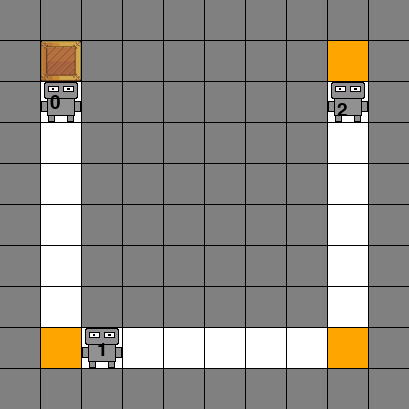
\includegraphics[width=0.154\textwidth]{figures/moving_company_1.png}
  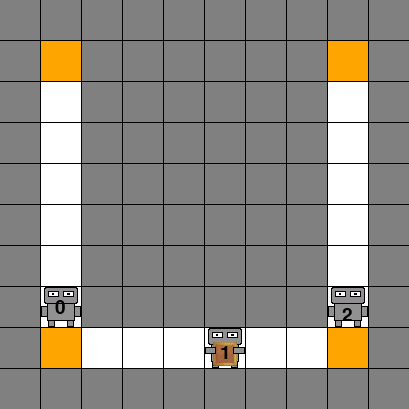
\includegraphics[width=0.154\textwidth]{figures/moving_company_2.png}
  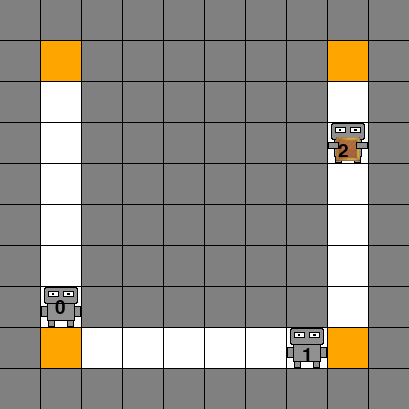
\includegraphics[width=0.154\textwidth]{figures/moving_company_3.png}
  \caption{Rendus visuels de \emph{Moving Company} avec trois agents déménageurs et un paquet.}
  \label{fig:env_moving_company}
\end{figure}
%
Le code de \emph{PRAHOM Wrapper} utilisé pour \emph{Moving Company} est résumé dans \autoref{lst:wrapper_mc}.

\paragraph{Mise en place et configuration}

Dans cette phase nous préparons notre utilisation de \emph{PRAHOM Wrapper} (cases jaunes dans \autoref{fig:prahom_wrapper_technical_view}).
Après avoir instancié l'environnement \emph{Moving Company} (ligne 3), nous définissions quelques relations connues entre des sous-historiques et des spécifications organisationnelles connues (ligne 4). De même nous définissons des contraintes d'organisation (ligne 5). Ensuite, \emph{PRAHOM Wrapper} enveloppe l'environnement avec les éventuelles relations et les contraintes préétablies (ligne 6). Les contraintes et relations peuvent être des mapping ou des fonctions dans la mesure où les deux associent respectivement un agent à ses contraintes et un historique à des spécifications organisationnelles connues.

Le concepteur peut aussi modifier les valeurs par défaut relatives aux modes de respect des contraintes, aux méthodes utilisées pour l'analyse des historiques, aux différentes spécifications organisationnelles attendues, et aux figures et supports associés aux spécifications générées.

\paragraph{Entraînement contraint des agents}

Le concepteur peut ensuite procéder classiquement à l'apprentissage avec l'environnement enveloppé. Sinon il peut utiliser l'algorithme PPO integré (case verte dans \autoref{fig:prahom_wrapper_technical_view}). Nous utilisons cette fonctionnalité (ligne 7) avec le paramétrage existant \textquote{PPO\_default} : un nombre d'itérations indéfini, un temps d'apprentissage de 2h, le mode apprentissage centralisé et exécution décentralisée, pas d'optimisation des hyper-paramètres, la sauvegarde de la meilleure politique et la restauration à partir du dernier checkpoint s'il existe.
\emph{PRAHOM Wrapper} permet alors d'obliger les agents à respecter la contrainte donnée (ligne 5). Ici, si l'\textquote{agent\_0} observe qu'un paquet se trouve dans la case supérieure à la sienne, il doit prendre le paquet (action $5$).

\paragraph{Génération et évaluation des spécifications organisationnelles }

Nous générons ensuite les spécifications organisationnelles (case bleue dans \autoref{fig:prahom_wrapper_technical_view}) avec le profil par défaut. Cela génère et analyse des historiques conjoints joués sur 5 épisodes avec la meilleure politique apprise (ligne 8).
\emph{PRAHOM Wrapper} prend en priorité en compte les relations déjà connues (ligne 4): si on voit que l'historique d'un agent contient l'action $3$ (se déplacer à gauche) alors cet agent a le rôle \textquote{horizontal\_mover}.

Sans relation entre historiques et spécifications organisationnelles préétablies, \emph{PRAHOM Wrapper} infère ces dernières d'après les définitions générales données. Ainsi, un rôle peut être inféré par mesure de similarité entre les historiques selon plusieurs façons complémentaires : par clustering de séquence (lié à un dendrogramme) ; par recherche des K-voisins les plus proches (lié à une ACP des historiques) ; par analyse statistique (fréquence, variance des actions liées à diverses visualisations) ; etc.
Des techniques sont également utilisées pour inférer des objectifs : analyse de fréquence des observations communes des agents avec un même rôle ; analyse des états seuils récurrents déclenchant une amélioration notable de l'évolution de la récompense (lié à un graphe de transition d'états).

À partir des rôles et objectifs obtenus, \emph{PRAHOM Wrapper} infère d'autres spécifications organisationnelles comme les compatibilités entre rôles, les permissions et obligations. Il résulte les spécifications propres à l'organisation (ligne 8).

\begin{lstlisting}[language=Python, caption={Utilisation synthétique de \emph{PRAHOM Wrapper} pour \emph{Moving Company}}, label={lst:wrapper_mc}]
from custom_envs.movingcompany import moving_company_v0
from prahom_wrapper import prahom_wrapper
env = moving_company_v0.parallel_env(render_mode="human")
hist_to_specs = lambda hist: {"role": "horizontal_mover"} if "3" in [act for obs, act in hist.items()] else None
agt_to_cons_specs = {"agent_0": {"[0 5 0 0 2 0 0 1 0]": 5}}
env = prahom_wrapper(env, hist_to_specs, agt_to_cons_specs, "CORRECT", ["sequence_clustering"], ["role", "goals"], ["dendogram", "PCA"])
env.train("PPO_default")
raw_specs = env.generate_specs()
\end{lstlisting}

\section{Conclusion}

\emph{PRAHOM Wrapper} donne des moyens de contraindre l'apprentissage des agents et déterminer automatiquement les spécifications organisationnelles sur la base d'historiques en étant ainsi agnostique de l'algorithme MARL.
La version actuelle met en jeu de premières techniques statistiques simples et d'apprentissage non supervisé pour l'analyse des historiques pour identifier des spécifications organisationnelles.

Cependant, ces techniques présentent des limitations pour l'identification des liens entre rôles (communications, représentations) menant à des spécifications incomplètes.
Les travaux de l'apprentissage hiérarchique sont susceptibles d'aider à caractériser les organisations émergentes au long de l’apprentissage de façon plus complète.
À terme, nous visons également à améliorer l'applicabilité de \emph{PRAHOM Wrapper} en enrichissant son interface et son intégration dans des contextes industriels et de recherche.


% \begin{thebibliography}{9}
% {\small
% \bibitem{bar} U. Nexpert, \emph{Le livre,} Son Editeur, 1929.

% \bibitem{foo} I. Troiseu-Pami, Un article intéressant, \emph{Journal de
%     Spirou}, Vol. 17, pp. 1-100, 1987
% }
% \end{thebibliography}

% \section*{Remerciements}

% Ce travail est financé par Thales Land Air Systems dans le cadre des travaux conjoints de la chair Cyb'Air et de l'AICA IWG.

\section*{References}
\small
\bibliographystyle{abbrv}
\bibliography{references}


\end{document}

%%% Local Variables: 
%%% mode: latex
%%% TeX-SMAter: "jfsmaLatex"
%%% ispell-local-dictionary: "francais"
%%% TeX-command-extra-options: "-shell-escape"
%%% End: 